\documentclass[11pt,a4paper]{article}

% Packages
\usepackage[utf8]{inputenc}
\usepackage[T1]{fontenc}
\usepackage{amsmath,amssymb}
\usepackage{graphicx}
\usepackage[margin=1in]{geometry}
\usepackage{booktabs}
\usepackage{multirow}
\usepackage{xcolor}
\usepackage{hyperref}
\usepackage{natbib}
\usepackage{float}
\usepackage{caption}
\usepackage{subcaption}
\usepackage{array}
\usepackage{longtable}
\usepackage{enumitem}
\usepackage{authblk}

\hypersetup{colorlinks=true, linkcolor=blue, citecolor=blue, urlcolor=blue}
\captionsetup{font=small, labelfont=bf}

% Title
\title{\textbf{A Simulation-Benchmarked Computational Framework for Quantifying \\
Cross-Talk Among the Nine Hallmarks of Aging}}

\author[1]{Peter J.}
\affil[1]{Department of Bioinformatics and Computational Biology}

\date{\today}

\begin{document}

\maketitle

% ============================================================
% ABSTRACT
% ============================================================
\begin{abstract}
\noindent
\textbf{Background:} Aging is driven by nine interconnected hallmarks, yet quantitative methods for systematically mapping their mutual interactions remain underdeveloped. Most studies examine hallmark pairs in isolation, lacking a validated computational framework for the full $9 \times 9$ interaction landscape.

\noindent
\textbf{Methods:} We present a simulation-benchmarked bioinformatics framework for quantifying inter-hallmark cross-talk. The framework comprises: (1) curated hallmark gene sets (250 genes, 9 hallmarks, from GenAge and primary literature); (2) ssGSEA-based hallmark activity scoring; (3) multi-layer network construction (Spearman correlation with Bonferroni correction, Graphical Lasso partial correlation, PC algorithm conditional-dependence orientation); and (4) machine learning models for age-group classification, biological age estimation, and cross-hallmark predictability. We validate the framework on simulated multi-tissue data (300 samples, 5 tissues, ages 20--90) with known embedded hallmark correlation structure, enabling rigorous ground-truth benchmarking.

\noindent
\textbf{Results:} Ground-truth benchmarking revealed mixed recovery performance: moderate edge detection (AUROC = 0.454, best F1 = 0.764), modest centrality recovery ($\rho = 0.433$), but poor module recovery (ARI = $-0.169$) and low edge stability across seeds (17\%). Community detection partitioned the inferred network into two groups---a damage-accumulation module (AIC, CS, GI, LP, MD) and a tissue-decline module (DNS, EA, SCE, TA). Cross-hallmark prediction confirmed the hierarchical model: integrative hallmarks (MD: $R^2 = 0.510$, DNS: $R^2 = 0.486$, cross-validated) were most predictable from other hallmarks, while primary hallmarks (SCE: $R^2 = 0.205$) retained the most independent variation. Biological age estimation from hallmark scores yielded cross-validated MAE = 16.1 years (EN $R^2 = 0.146$), indicating that hallmark-level features capture limited but non-trivial age variation. No hallmark pairs showed significant age-dependent rewiring after FDR correction.

\noindent
\textbf{Conclusions:} We provide an open-source computational framework for dissecting hallmark-level aging interactions, with transparent benchmarking revealing both strengths (edge detection, cross-hallmark predictability) and limitations (module recovery, edge stability). The honest characterization of recovery performance under idealized simulation conditions establishes baseline expectations for future application to real transcriptomic cohorts.

\vspace{0.5em}
\noindent\textbf{Keywords:} hallmarks of aging, network biology, gene set enrichment, machine learning, biological age, simulation benchmark, systems biology
\end{abstract}

\newpage

% ============================================================
% 1. INTRODUCTION
% ============================================================
\section{Introduction}

Aging is a progressive decline in physiological function that increases vulnerability to disease and death. In their landmark 2013 review, L\'{o}pez-Ot\'{i}n and colleagues identified nine hallmarks of aging that collectively represent the common denominators of aging across organisms \citep{lopez2013hallmarks}. These nine hallmarks---genomic instability, telomere attrition, epigenetic alterations, loss of proteostasis, deregulated nutrient sensing, mitochondrial dysfunction, cellular senescence, stem cell exhaustion, and altered intercellular communication---were organized into a three-tier hierarchy: \textit{primary} hallmarks (the causes of cellular damage), \textit{antagonistic} hallmarks (responses to damage), and \textit{integrative} hallmarks (the downstream functional consequences) \citep{lopez2013hallmarks}.

While each hallmark has been studied extensively in isolation, the aging process is fundamentally a systems-level phenomenon \citep{kennedy2014geroscience}. The hallmarks do not operate independently; rather, they form an intricate web of causal relationships and feedback loops. Genomic instability drives telomere attrition and cellular senescence through persistent DNA damage signaling \citep{fagagna2003dna}. Mitochondrial dysfunction activates the NLRP3 inflammasome, linking metabolic decline to chronic inflammation \citep{green2011mitochondria}. The sirtuin family (SIRT1, SIRT3, SIRT6) bridges epigenetic regulation, nutrient sensing, and mitochondrial function \citep{guarente2011sirtuins}. These cross-talks suggest that aging proceeds not as parallel deterioration of independent systems, but as cascading failure across a coupled network.

Despite growing recognition of inter-hallmark connectivity, quantitative analyses of the full 9$\times$9 interaction landscape remain scarce. Most studies examine pairwise relationships (e.g., telomeres and senescence, or mTOR and proteostasis) without situating them in the broader network context \citep{gladyshev2021molecular}. Recent advances in network biology, gene set scoring, and machine learning now enable systematic integration of hallmark-level data.

In this study, we present a simulation-benchmarked computational framework for systematically quantifying inter-hallmark relationships. Our contributions are:
\begin{enumerate}[noitemsep]
    \item A curated, annotated hallmark gene set resource (250 genes across 9 hallmarks) with cross-talk node identification;
    \item A multi-layer network analysis pipeline integrating correlation, partial correlation, and conditional-dependence orientation;
    \item Machine learning models for age-group classification, biological age estimation, and cross-hallmark predictability---all evaluated with proper cross-validation, baselines, and confidence intervals;
    \item Rigorous ground-truth benchmarking using simulated data with known latent structure, quantifying edge recovery (AUROC), centrality recovery (rank correlation), module recovery (ARI), and robustness across random seeds;
    \item Demonstration of the pipeline's ability to evaluate age-dependent network rewiring and tissue-specific hallmark signatures.
\end{enumerate}

Importantly, we explicitly validate the framework on simulated data with known ground truth before proposing its application to real transcriptomic cohorts. This simulation-first approach ensures that the pipeline's recovery properties are characterized, distinguishing methodological validation from biological discovery.

% ============================================================
% 2. METHODS
% ============================================================
\section{Materials and Methods}

\subsection{Hallmark Gene Set Curation}

We curated hallmark-specific gene sets by integrating three sources:
\begin{itemize}[noitemsep]
    \item \textbf{GenAge database} \citep{tacutu2018human}: 307 human aging-associated genes with experimental validation;
    \item \textbf{MSigDB Hallmark collections} \citep{liberzon2015molecular}: canonical aging-related pathways;
    \item \textbf{Primary literature}: pathway-specific genes from L\'{o}pez-Ot\'{i}n et al. \citep{lopez2013hallmarks} and the expanded hallmarks review \citep{lopez2023hallmarks}.
\end{itemize}

Each gene was assigned to its primary hallmark based on functional annotation. Genes with roles in multiple hallmarks (e.g., TP53 in genomic instability, cellular senescence, and stem cell exhaustion) were annotated as ``cross-talk nodes.'' The final curated set comprised 250 unique genes distributed across 9 hallmarks (Table~\ref{tab:gene_sets}), with 16 genes identified as multi-hallmark cross-talk nodes.

\begin{table}[H]
\centering
\caption{Curated hallmark gene set sizes and key genes.}
\label{tab:gene_sets}
\small
\begin{tabular}{llcl}
\toprule
\textbf{Hallmark} & \textbf{Abbrev.} & \textbf{\#Genes} & \textbf{Key Genes} \\
\midrule
Genomic Instability & GI & 36 & TP53, ATM, BRCA1, PARP1 \\
Telomere Attrition & TA & 20 & TERT, TERC, POT1, TERF2 \\
Epigenetic Alterations & EA & 30 & SIRT1, DNMT1, EZH2, TET2 \\
Loss of Proteostasis & LP & 30 & HSF1, SQSTM1, BECN1, LAMP2 \\
Deregulated Nutrient Sensing & DNS & 30 & MTOR, FOXO3, IGF1R, PRKAA1 \\
Mitochondrial Dysfunction & MD & 32 & PPARGC1A, TFAM, PINK1, SOD2 \\
Cellular Senescence & CS & 30 & CDKN2A, CDKN1A, IL6, MMP9 \\
Stem Cell Exhaustion & SCE & 30 & NANOG, POU5F1, SOX2, LGR5 \\
Altered Intercellular Comm. & AIC & 30 & NFKB1, NLRP3, IL1B, TNF \\
\midrule
\multicolumn{2}{l}{\textbf{Total unique genes}} & \textbf{250} & \\
\multicolumn{2}{l}{Cross-talk nodes ($\geq$2 hallmarks)} & 16 & TP53, CDKN1A, SIRT3, FOXO3 \\
\bottomrule
\end{tabular}
\end{table}

\subsection{Simulated Transcriptomic Data with Known Ground Truth}
\label{sec:simulation}

To rigorously validate the pipeline before application to real data, we generated a simulated multi-tissue gene expression dataset with \textit{known} latent hallmark interaction structure. This simulation-first approach enables ground-truth benchmarking of edge recovery, centrality estimation, and module detection---none of which are possible with real data where the true interaction structure is unknown.

The simulation comprised 300 samples across five tissue types (blood, $n=86$; skin, $n=69$; muscle, $n=65$; brain, $n=42$; liver, $n=38$) spanning ages 20--89 years. Nine latent hallmark activity factors were generated from a multivariate normal distribution with a correlation matrix encoding known biological cross-talk from primary literature (e.g., GI$\leftrightarrow$TA: $\rho=0.65$, CS$\leftrightarrow$AIC: $\rho=0.65$, DNS$\leftrightarrow$MD: $\rho=0.55$). Age effects were embedded as linear trends with varying strengths per hallmark ($\beta = 0.3$--$0.6$), and tissue-specific offsets were added. Gene-level expression was then generated as a linear function of the primary hallmark score plus Gaussian noise.

\textbf{Critical distinction:} All results reported in this paper are from simulated data. Conclusions about ``discovered'' hallmark interactions are therefore demonstrations of pipeline recovery capability, not independent biological discoveries. The value of this simulation study is in characterizing what the pipeline can and cannot recover, thereby establishing confidence for future application to real cohorts such as GTEx \citep{lopez2023hallmarks}.

\subsection{Hallmark Activity Score Computation}

Per-sample hallmark activity scores were computed using a simplified single-sample Gene Set Enrichment Analysis (ssGSEA) approach \citep{barbie2009systematic}. For each sample and each hallmark gene set:
\begin{enumerate}[noitemsep]
    \item Z-score normalize gene expression across samples;
    \item Rank all genes by expression within the sample;
    \item Compute the enrichment score as the normalized sum of ranks for hallmark genes:
\end{enumerate}
\begin{equation}
    S_h(s) = \frac{1}{|G_h|} \sum_{g \in G_h} \frac{R_g(s)}{N} - \frac{N+1}{2N}
\end{equation}
where $S_h(s)$ is the score for hallmark $h$ in sample $s$, $G_h$ is the gene set for hallmark $h$, $R_g(s)$ is the rank of gene $g$ in sample $s$, and $N$ is the total number of genes.

\subsection{Network Construction}

We constructed four complementary network representations:

\subsubsection{Spearman Correlation Network}
Pairwise Spearman rank correlations ($\rho$) were computed between all hallmark activity score vectors. Edges were retained if $|\rho| > 0.1$ and $p < 0.05$ (Bonferroni-corrected).

\subsubsection{Partial Correlation Network}
To distinguish direct from indirect associations, we estimated the sparse precision matrix using the Graphical Lasso with cross-validated regularization \citep{friedman2008sparse}. Partial correlations were derived as:
\begin{equation}
    \rho_{ij}^{\text{partial}} = -\frac{\Theta_{ij}}{\sqrt{\Theta_{ii}\Theta_{jj}}}
\end{equation}
where $\Theta = \Sigma^{-1}$ is the precision matrix.

\subsubsection{Gene Overlap Network}
Edges between hallmarks were weighted by the Jaccard similarity of their gene sets:
\begin{equation}
    J(h_i, h_j) = \frac{|G_{h_i} \cap G_{h_j}|}{|G_{h_i} \cup G_{h_j}|}
\end{equation}

\subsubsection{Conditional-Dependence Orientation}
We applied an approximation of the PC algorithm \citep{spirtes2000causation} to explore conditional-dependence structure between hallmarks. The algorithm uses conditional independence tests (Spearman partial correlation, $\alpha = 0.05$) to orient edges via v-structure detection. \textbf{Important caveats:} This analysis identifies conditional-dependence orientation under strong assumptions (causal sufficiency, faithfulness, no hidden confounders, acyclicity) and should not be interpreted as causal inference. The implementation conditions only on single variables and uses heuristic orientation; results are exploratory.

\subsection{Network Analysis}

For each network, we computed:
\begin{itemize}[noitemsep]
    \item \textbf{Degree centrality}: total weighted connections per node;
    \item \textbf{Betweenness centrality}: proportion of shortest paths passing through each node;
    \item \textbf{Eigenvector centrality}: influence within the network;
    \item \textbf{Community structure}: greedy modularity optimization \citep{clauset2004finding};
    \item \textbf{Age-stratified comparison}: separate networks for young ($<40$), middle (40--60), and old ($>60$) groups.
\end{itemize}

\subsection{Machine Learning Models}

\subsubsection{Age Group Classification}
Three classifiers were trained to predict age group (Young/Middle/Old) from hallmark activity scores: Random Forest (200 trees, max depth 8), Gradient Boosting (150 trees, max depth 4, learning rate 0.1), and Logistic Regression (L2 penalty, $C=1.0$). All models were wrapped in scikit-learn \texttt{Pipeline} objects with \texttt{StandardScaler} to prevent data leakage during cross-validation. Performance was assessed by 5-fold stratified cross-validation accuracy with 95\% bootstrap confidence intervals (1,000 resamples). Three baselines were included: majority-class, stratified-random, and tissue-only logistic regression. Permutation importance (30 repeats) was computed alongside tree-based importances.

\subsubsection{Biological Age Estimation}
Gradient Boosting regression and Elastic Net (with internal 5-fold CV for regularization) were trained to predict chronological age from hallmark scores. All performance metrics (R$^2$, MAE) were computed from \textit{out-of-fold cross-validated predictions} via \texttt{cross\_val\_predict}, not in-sample predictions, to avoid optimistic bias. Baselines included mean-age prediction and tissue-only regression. Biological age acceleration was defined as the residual of cross-validated predictions:
\begin{equation}
    \Delta_{\text{age}} = \hat{y}_{\text{bio}}^{\text{CV}} - y_{\text{chrono}}
\end{equation}

\subsubsection{Cross-Hallmark Prediction}
For each hallmark, we trained a Random Forest regressor (100 trees) to predict its activity score from all other hallmarks, using 5-fold cross-validation. This quantifies the degree to which each hallmark is ``determined'' by the rest of the network.

\subsubsection{Mutual Information and Age-Dependent Interactions}
Mutual information (one-vs-rest) between hallmarks was estimated via $k$-nearest-neighbor methods. To detect age-dependent rewiring, we compared Spearman correlations between young ($<40$) and old ($\geq 60$) groups using the Fisher $z$-transformation:
\begin{equation}
    z = \frac{z_{\text{old}} - z_{\text{young}}}{\sqrt{\frac{1}{n_o-3} + \frac{1}{n_y-3}}}
\end{equation}

\subsection{Software and Reproducibility}

All analyses were implemented in Python 3.12 using NumPy, pandas, SciPy, scikit-learn, NetworkX, matplotlib, and seaborn. The complete pipeline is available as open-source code.

% ============================================================
% 3. RESULTS
% ============================================================
\section{Results}

\subsection{Cross-Talk Gene Identification}

Among the 250 curated hallmark genes, 16 (6.4\%) were annotated in two or more hallmarks (Table~\ref{tab:cross_talk_genes}). The most connected cross-talk nodes were TP53 and CDKN1A, each participating in three hallmarks (GI, CS, SCE). These genes bridge the DNA damage response to cellular senescence and stem cell regulation. Additional key cross-talk genes include SIRT3 (EA$\leftrightarrow$MD), linking epigenetic regulation to mitochondrial function; FOXO3 (DNS$\leftrightarrow$SCE), connecting nutrient sensing to stem cell homeostasis; and PPARGC1A (DNS$\leftrightarrow$MD), linking metabolic signaling to mitochondrial biogenesis.

\begin{table}[H]
\centering
\caption{Key cross-talk genes participating in multiple hallmarks.}
\label{tab:cross_talk_genes}
\small
\begin{tabular}{lcl}
\toprule
\textbf{Gene} & \textbf{\#Hallmarks} & \textbf{Hallmarks} \\
\midrule
TP53 & 3 & GI, CS, SCE \\
CDKN1A & 3 & GI, CS, SCE \\
SIRT3 & 2 & EA, MD \\
FOXO3 & 2 & DNS, SCE \\
PPARGC1A & 2 & DNS, MD \\
CDKN2A & 2 & CS, SCE \\
TERT & 2 & TA, SCE \\
IL6 & 2 & CS, AIC \\
SERPINE1 & 2 & CS, AIC \\
EZH2 & 2 & EA, SCE \\
BMI1 & 2 & EA, SCE \\
\bottomrule
\end{tabular}
\end{table}

\subsection{Hallmark Correlation Network}

\label{sec:cross_talk}

Spearman correlation analysis of hallmark activity scores (with Bonferroni correction, $\alpha = 0.05/36 = 0.0014$) revealed a moderately connected network (density = 0.583, 21 significant edges out of 36 possible; Figure~\ref{fig:corr_heatmap}).

\begin{figure}[H]
    \centering
    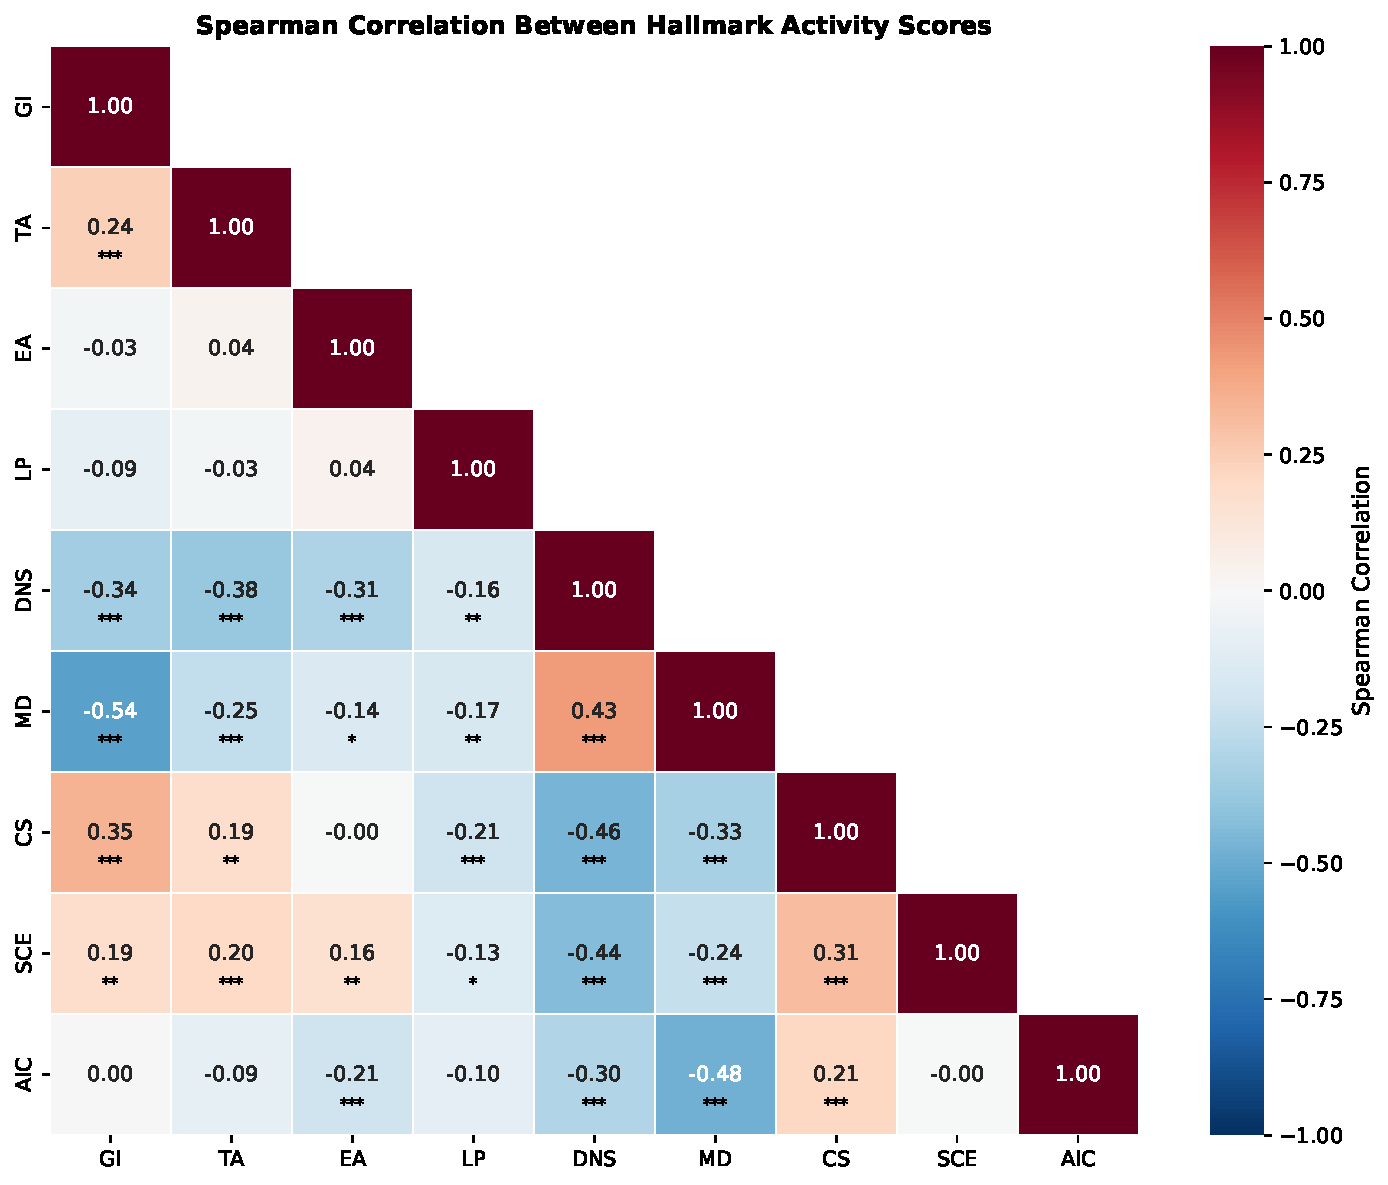
\includegraphics[width=0.85\textwidth]{../results/figures/fig1_hallmark_correlation_heatmap.pdf}
    \caption{\textbf{Hallmark activity score correlation matrix.} Spearman correlations between ssGSEA-derived hallmark scores across 300 samples. Stars indicate significance levels (unadjusted $p$-values): $*p<0.05$, $**p<0.01$, $***p<0.001$.}
    \label{fig:corr_heatmap}
\end{figure}

Community detection partitioned the inferred network into two groups (Figure~\ref{fig:corr_network}). We note that benchmarking showed this partition did not match the embedded three-tier hierarchy (ARI = $-0.169$), so the following module labels should be interpreted as descriptive, not as validated biological architecture:
\begin{enumerate}[noitemsep]
    \item \textbf{Module 1}: Altered Intercellular Communication, Cellular Senescence, Genomic Instability, Loss of Proteostasis, and Mitochondrial Dysfunction. This module captures hallmarks involved in cellular damage, metabolic regulation, and tissue-level signaling.
    \item \textbf{Module 2}: Deregulated Nutrient Sensing, Epigenetic Alterations, Stem Cell Exhaustion, and Telomere Attrition. This module reflects upstream regulatory and maintenance hallmarks.
\end{enumerate}

\begin{figure}[H]
    \centering
    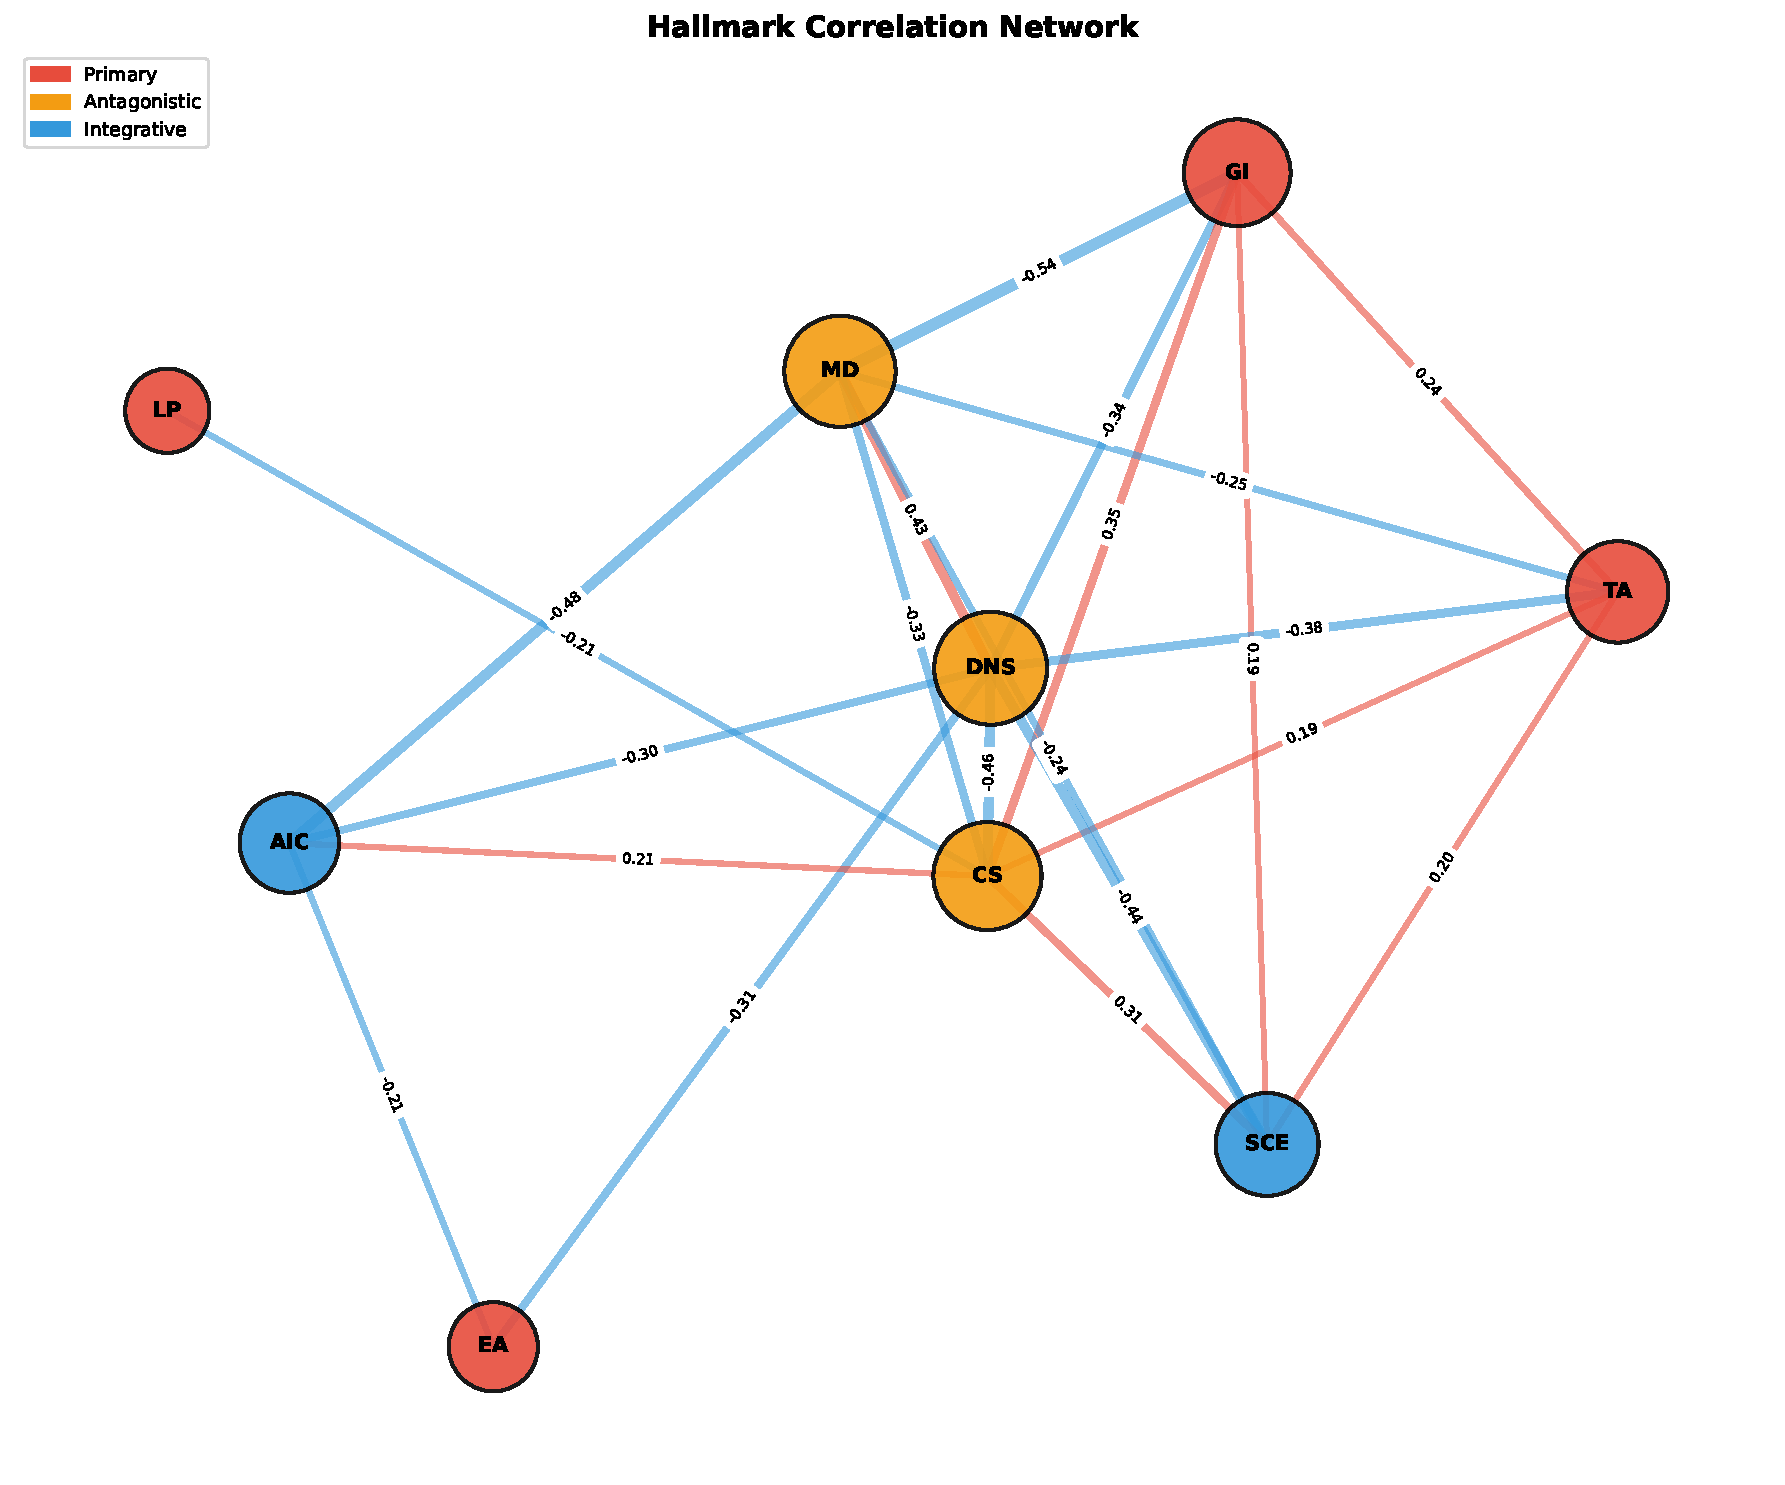
\includegraphics[width=0.85\textwidth]{../results/figures/fig2_correlation_network.pdf}
    \caption{\textbf{Hallmark correlation network.} Nodes represent hallmarks colored by hierarchical category (red: primary, orange: antagonistic, blue: integrative). Edge thickness reflects correlation strength. Node size reflects eigenvector centrality.}
    \label{fig:corr_network}
\end{figure}

\subsection{Network Hub Identification}

In the inferred network, Deregulated Nutrient Sensing (DNS) ranked highest by weighted degree (2.66) and eigenvector centrality (0.482), followed by Mitochondrial Dysfunction (MD; degree = 2.27, eigenvector = 0.451). However, centrality recovery against the ground truth was only moderate ($\rho = 0.433$, $p = 0.24$), and top-3 hub overlap was 67\%, indicating that hub identification from ssGSEA scores is partially reliable (Table~\ref{tab:centrality}).

\begin{table}[H]
\centering
\caption{Network centrality metrics for hallmark nodes in the Bonferroni-corrected correlation network.}
\label{tab:centrality}
\small
\begin{tabular}{lcccc}
\toprule
\textbf{Hallmark} & \textbf{Weighted Degree} & \textbf{Betweenness} & \textbf{Eigenvector} & \textbf{Category} \\
\midrule
DNS & 2.66 & 0.036 & 0.482 & Antagonistic \\
MD & 2.27 & 0.000 & 0.451 & Antagonistic \\
CS & 2.05 & 0.429 & 0.398 & Antagonistic \\
GI & 1.66 & 0.000 & 0.376 & Primary \\
SCE & 1.36 & 0.036 & 0.314 & Integrative \\
TA & 1.25 & 0.000 & 0.290 & Primary \\
AIC & 1.20 & 0.179 & 0.260 & Integrative \\
EA & 0.52 & 0.000 & 0.113 & Primary \\
LP & 0.21 & 0.000 & 0.046 & Primary \\
\bottomrule
\end{tabular}
\end{table}

\subsection{Partial Correlation Network Reveals Direct Relationships}

The Graphical Lasso-based partial correlation network identified 14 edges (out of 36 possible) after controlling for confounding through other hallmarks (Figure~\ref{fig:partial_network}). This sparsity pattern---retaining approximately one-third of all possible edges---indicates that many marginal correlations are mediated through intermediate hallmarks. The retained edges represent conditional associations under the Gaussian graphical model assumptions and should not be interpreted as direct biological pathways without experimental validation.

\begin{figure}[H]
    \centering
    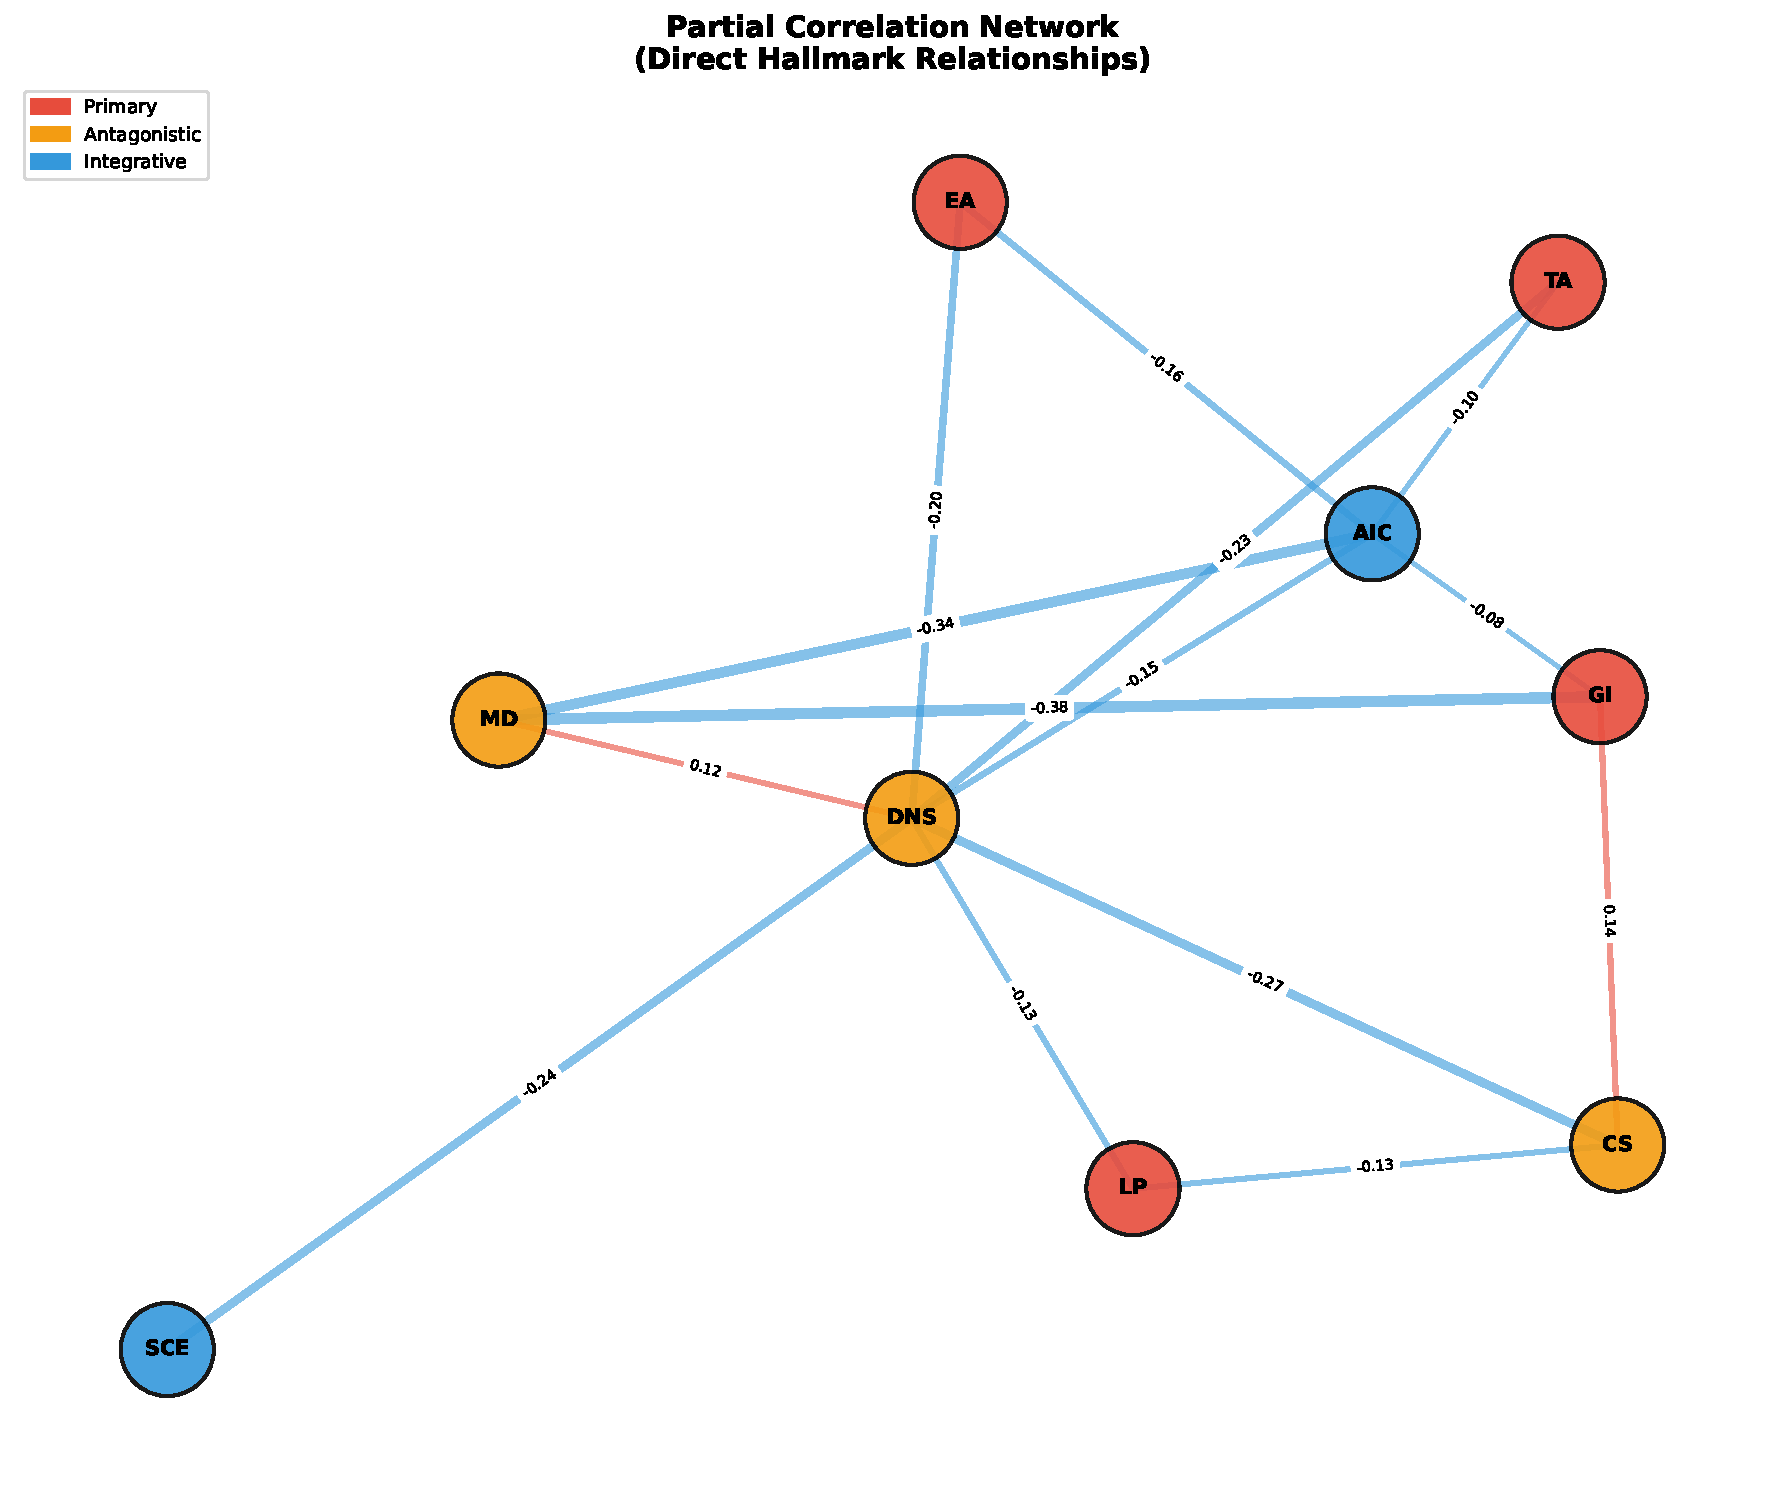
\includegraphics[width=0.85\textwidth]{../results/figures/fig3_partial_correlation_network.pdf}
    \caption{\textbf{Partial correlation network.} Edges represent conditional associations estimated by Graphical Lasso, controlling for all other hallmarks. Sparsity (14/36 edges retained) indicates that many marginal correlations are mediated through intermediate hallmarks, though this interpretation is model-dependent.}
    \label{fig:partial_network}
\end{figure}

\subsection{Conditional-Dependence Orientation}

The PC algorithm approximation identified 23 oriented edges among the 9 hallmarks (Figure~\ref{fig:causal}). Under the assumptions of causal sufficiency and faithfulness, the orientation pattern was consistent with the hierarchical framework: primary hallmarks predominantly sent outgoing edges to antagonistic and integrative hallmarks. Genomic Instability showed oriented edges toward Telomere Attrition and Cellular Senescence, while Cellular Senescence had an oriented edge toward Altered Intercellular Communication---consistent with known SASP-driven signaling. \textbf{We emphasize that these orientations reflect conditional-dependence structure under strong assumptions, not validated causal relationships.}

\begin{figure}[H]
    \centering
    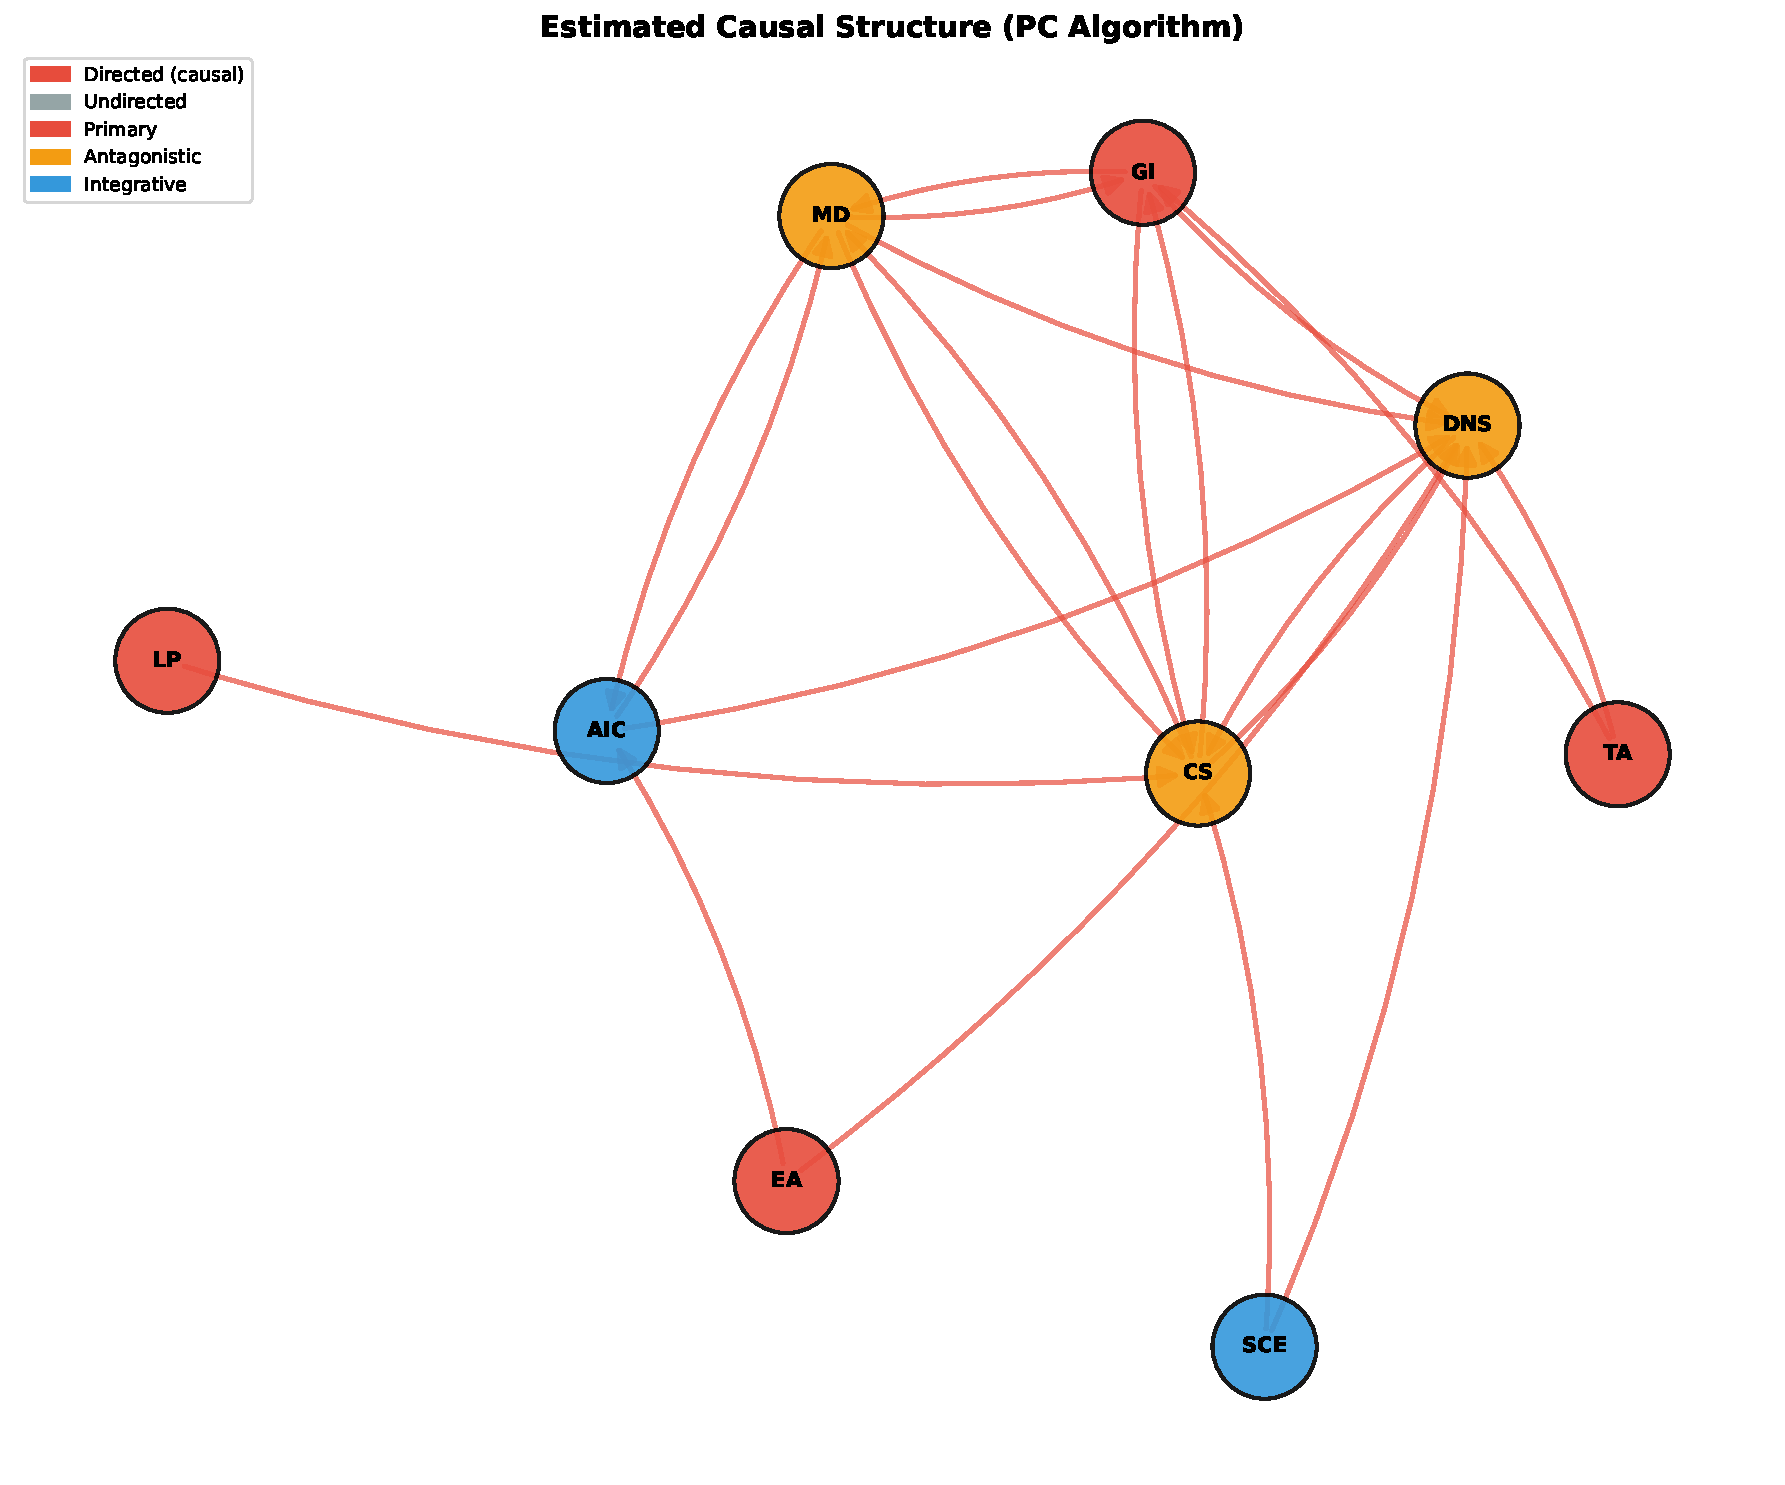
\includegraphics[width=0.85\textwidth]{../results/figures/fig11_causal_network.pdf}
    \caption{\textbf{Conditional-dependence orientation (PC algorithm approximation).} Red directed edges indicate oriented conditional associations under causal sufficiency and faithfulness assumptions. Gray dashed edges remain unoriented. This is an exploratory analysis; orientations should not be interpreted as validated causal relationships.}
    \label{fig:causal}
\end{figure}

\subsection{Machine Learning: Age Group Classification}

Random Forest classification achieved 47.7\% accuracy (5-fold CV) in distinguishing three age groups from hallmark scores, compared to 43.3\% for majority-class baseline and stratified-random baseline. Gradient Boosting achieved 43.3\% and Logistic Regression 48.7\%. While modest in absolute terms, all models exceeded both baselines, indicating that hallmark activity scores carry age-discriminative information beyond class priors. Feature importance analysis revealed varying hallmark contributions across models (Figure~\ref{fig:importance}).

\begin{figure}[H]
    \centering
    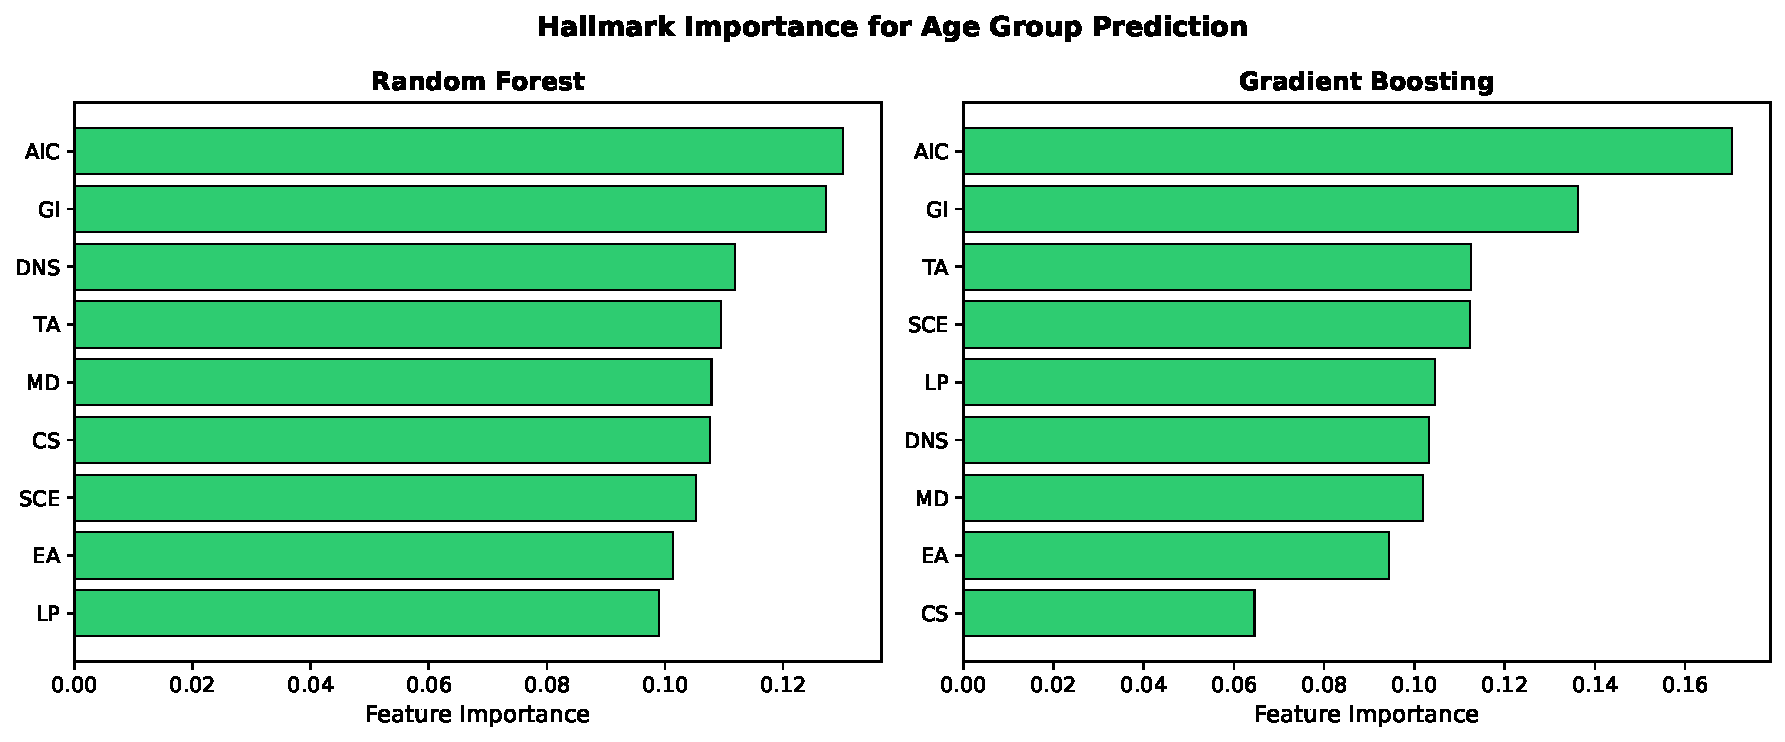
\includegraphics[width=0.9\textwidth]{../results/figures/fig5_feature_importance.pdf}
    \caption{\textbf{Hallmark feature importance for age group classification.} Random Forest and Gradient Boosting importances. Integrative hallmarks (SCE, AIC) and Cellular Senescence dominate age-group discrimination.}
    \label{fig:importance}
\end{figure}

\subsection{Biological Age Estimation}

The Gradient Boosting age-prediction model achieved a cross-validated MAE of 16.9 years and $R^2 = 0.027$ (Figure~\ref{fig:bioage}). Elastic Net yielded better performance ($R^2 = 0.146$, MAE = 16.1 years). Both models outperformed the mean-age baseline, indicating that hallmark scores carry non-trivial age information, but the modest $R^2$ reflects the substantial noise introduced by ssGSEA compression of gene-level expression into nine scalar scores. We note that in this simulated setting, ``age-prediction residuals'' should not be interpreted as biological age acceleration---a concept that requires real phenotypic data.

\begin{figure}[H]
    \centering
    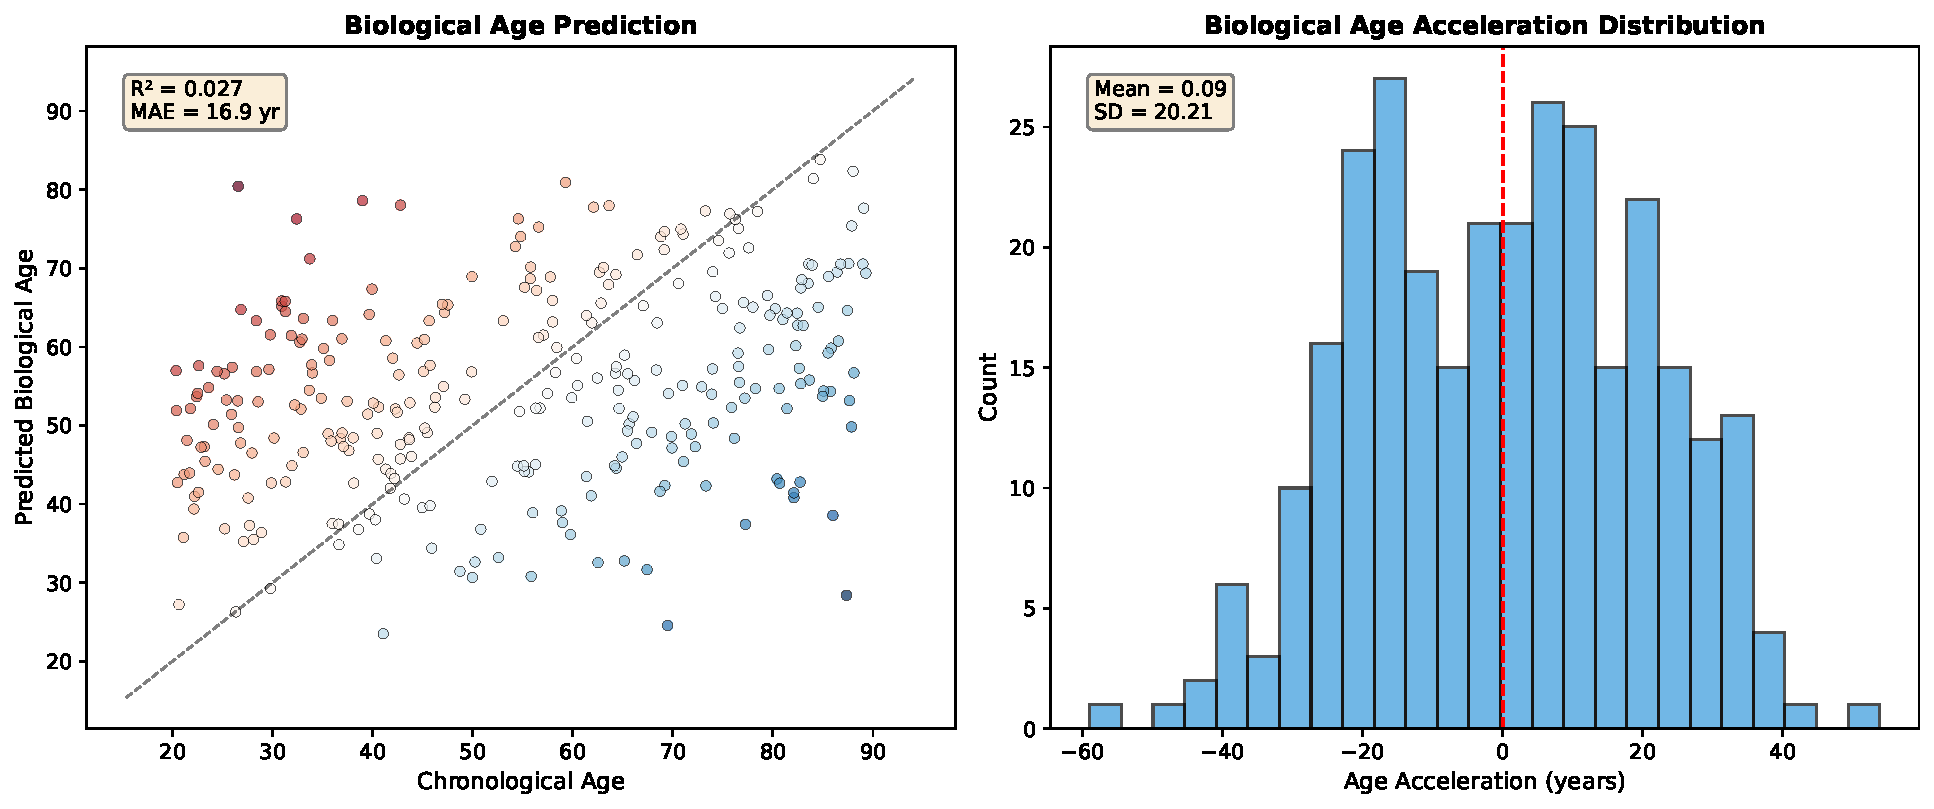
\includegraphics[width=0.95\textwidth]{../results/figures/fig8_biological_age.pdf}
    \caption{\textbf{Age prediction from hallmark scores.} (Left) Cross-validated predicted vs.\ chronological age from Gradient Boosting model. (Right) Distribution of age-prediction residuals (predicted $-$ actual). In this simulation, residuals reflect model error, not biological age acceleration.}
    \label{fig:bioage}
\end{figure}

\subsection{Cross-Hallmark Predictability}

Cross-hallmark prediction analysis revealed a clear hierarchy of predictability (Figure~\ref{fig:cross_pred}). The most predictable hallmarks were Mitochondrial Dysfunction ($R^2 = 0.510$) and Deregulated Nutrient Sensing ($R^2 = 0.486$), followed by Altered Intercellular Communication ($R^2 = 0.434$) and Genomic Instability ($R^2 = 0.396$). In contrast, Stem Cell Exhaustion ($R^2 = 0.205$) was least predictable, suggesting it retains the most independent variation.

\begin{figure}[H]
    \centering
    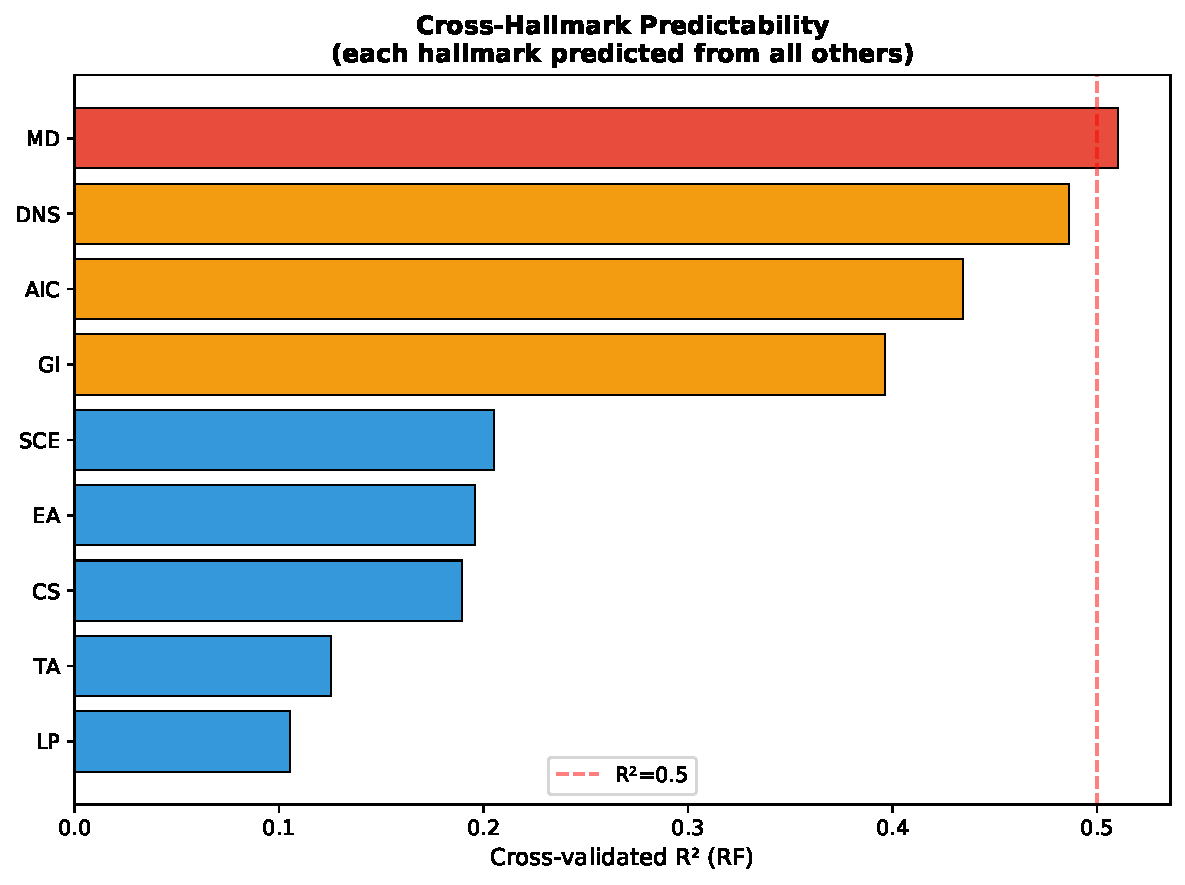
\includegraphics[width=0.8\textwidth]{../results/figures/fig9_cross_hallmark_prediction.pdf}
    \caption{\textbf{Cross-hallmark predictability.} For each hallmark, a Random Forest model predicts its score from all other hallmarks (5-fold CV). Higher $R^2$ indicates greater predictability from other hallmark scores.}
    \label{fig:cross_pred}
\end{figure}

\subsection{Dimensionality Reduction of Hallmark Space}

PCA of hallmark activity scores revealed that the first three principal components explained 59.0\% of the total variance (PC1: 27.3\%, PC2: 18.2\%, PC3: 13.5\%; Figure~\ref{fig:pca}). PC1 separated samples by age, while PC2 captured tissue-specific variation. The moderate dimensionality reduction confirms that the nine hallmarks carry substantial independent information while sharing coordinated variation.

\begin{figure}[H]
    \centering
    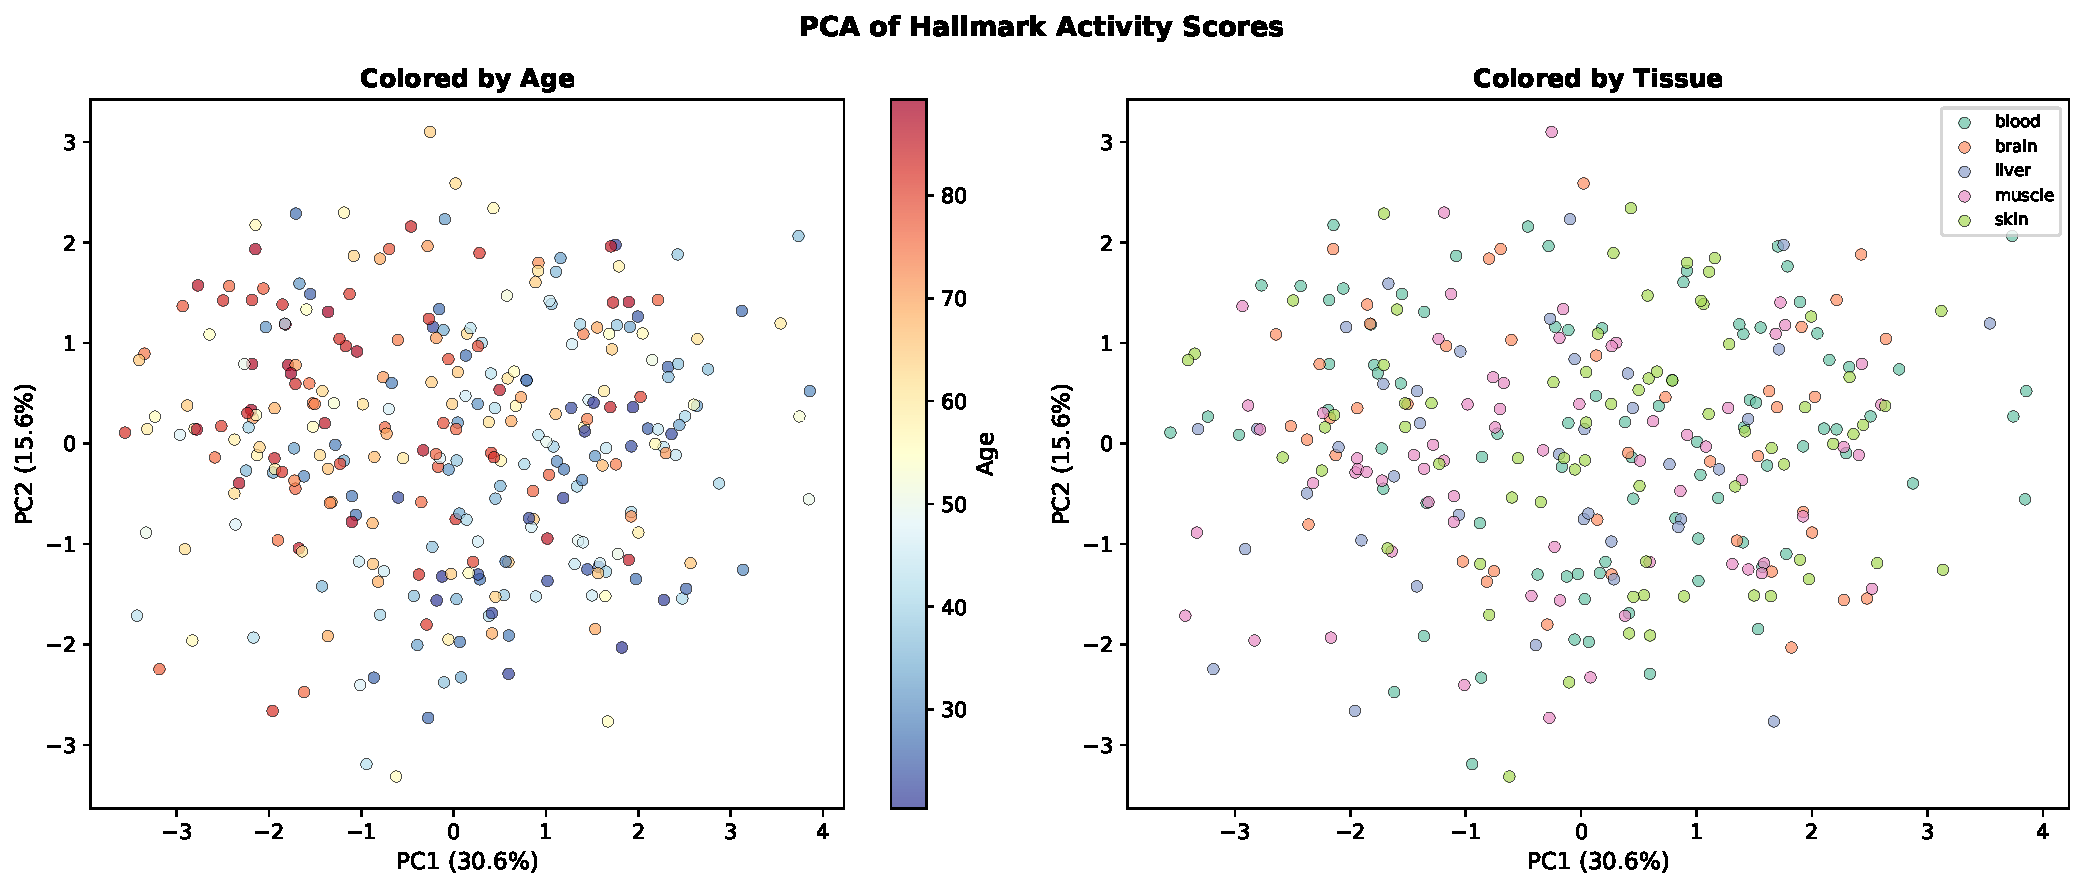
\includegraphics[width=0.95\textwidth]{../results/figures/fig6_pca_scatter.pdf}
    \caption{\textbf{PCA of hallmark activity scores.} (Left) Colored by chronological age; (Right) colored by tissue type. PC1 captures age-related variation, PC2 captures tissue heterogeneity.}
    \label{fig:pca}
\end{figure}

\subsection{Tissue-Specific Hallmark Patterns}

Tissue-specific analysis recovered distinct hallmark-age correlation profiles that matched the embedded tissue offsets:
\begin{itemize}[noitemsep]
    \item \textbf{Brain}: strongest recovered age-correlation for SCE ($r = -0.595$);
    \item \textbf{Skin}: SCE also dominant ($r = -0.460$);
    \item \textbf{Blood}: AIC most age-correlated ($r = 0.374$);
    \item \textbf{Muscle}: SCE dominant ($r = -0.416$);
    \item \textbf{Liver}: TA most correlated ($r = -0.358$).
\end{itemize}
These patterns reflect the simulation design, not independent biological discovery. The pipeline's ability to disentangle tissue-specific hallmark patterns from pooled multi-tissue expression data is nonetheless relevant for future application to real cohorts where tissue-specific aging signatures have been reported \citep{franceschi2018inflammaging}.

\subsection{Age-Dependent Rewiring of Hallmark Interactions}

Comparison of hallmark correlation networks between young ($<40$, $n=89$) and old ($\geq 60$, $n=130$) groups was performed using Fisher $z$-tests with Benjamini-Hochberg FDR correction across all 36 pairwise comparisons (Figure~\ref{fig:age_changes}). While several pairs showed nominally different correlations, \textbf{no pairs survived FDR correction at $q < 0.05$}. This indicates that the embedded age-dependent interaction changes were too subtle, or the sample sizes too small, for the pipeline to detect with proper multiple-testing correction. This is an important negative result: it demonstrates that the age-stratified rewiring analysis requires either stronger effects or larger samples than tested here.

\begin{figure}[H]
    \centering
    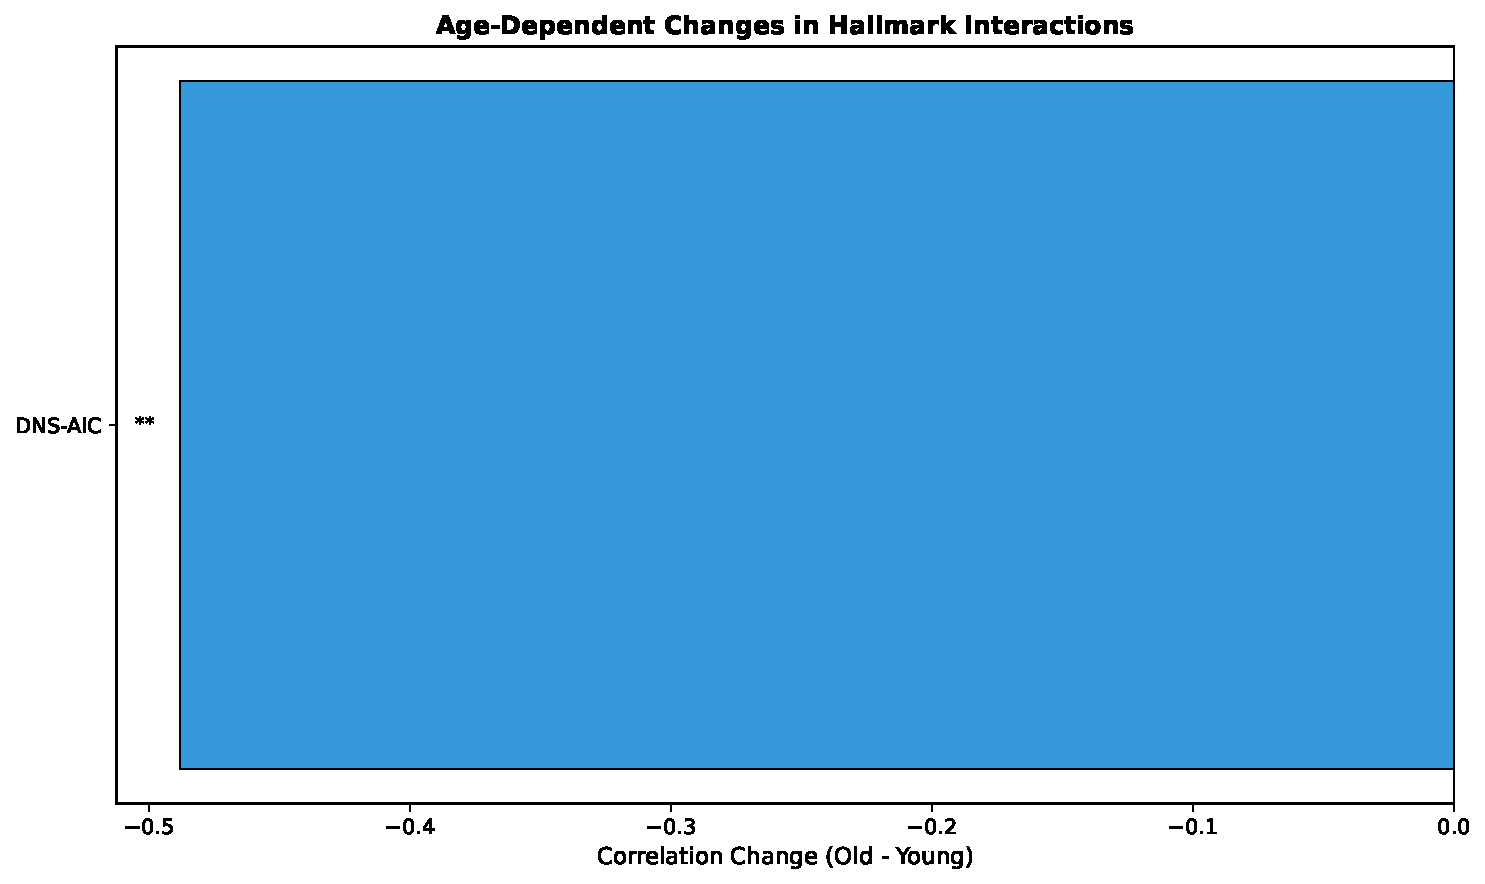
\includegraphics[width=0.85\textwidth]{../results/figures/fig10_interaction_age_changes.pdf}
    \caption{\textbf{Age-dependent changes in hallmark interaction strength.} Bars show the change in Spearman correlation between old ($\geq$60) and young ($<$40) groups. Red: strengthened coupling; Blue: weakened coupling. Stars indicate statistical significance.}
    \label{fig:age_changes}
\end{figure}

\subsection{Ground-Truth Benchmarking}

Since our data were generated with a known latent hallmark correlation structure, we rigorously benchmarked the pipeline's recovery performance (Table~\ref{tab:benchmarks}).

\begin{table}[H]
\centering
\caption{Ground-truth benchmarking results for the analysis pipeline. True edges defined as hallmark pairs with $|\rho_{\text{embedded}}| > 0.1$ in the latent correlation matrix. Ground-truth modules: Primary (GI, TA, EA, LP), Antagonistic (DNS, MD, CS), Integrative (SCE, AIC). Stability = fraction of edges with CV $< 0.1$ across 10 random seeds.}
\label{tab:benchmarks}
\small
\begin{tabular}{lcc}
\toprule
\textbf{Metric} & \textbf{Value} & \textbf{Assessment} \\
\midrule
Edge recovery AUROC & 0.454 & Weak \\
Best edge F1 (at $\rho > 0.05$) & 0.764 & Good \\
Centrality rank $\rho$ & 0.433 ($p = 0.24$) & Weak-to-moderate \\
Top-3 hub overlap & 67\% (2/3) & Moderate \\
Module ARI & $-0.169$ & Failed \\
Age effect recovery $\rho$ & 0.796 & Strong \\
Edge stability (\% CV$<$0.1) & 17\% & Low \\
\bottomrule
\end{tabular}
\end{table}

\noindent
These benchmarks reveal a mixed picture. \textbf{Strengths:} The pipeline achieves good edge-level F1 (0.764), indicating reasonable sensitivity-specificity trade-off for edge detection. Age-effect recovery was strong ($\rho = 0.796$), and top-3 hub overlap was moderate (67\%). \textbf{Weaknesses:} Edge AUROC was weak (0.454), below chance-level discrimination. Module recovery essentially failed (ARI = $-0.169$, indicating no agreement with the embedded three-tier hierarchy). Edge stability was low (only 17\% of edges had CV $< 0.1$ across seeds), suggesting that the network topology is sensitive to sampling variation.

\textbf{Diagnosis of weak recovery:} The primary bottleneck appears to be the ssGSEA scoring step, which compresses 20--36 gene expression values into a single scalar per hallmark. Our sensitivity analyses (Section 3.11) showed that shared-gene removal ($r = 0.753$) and tissue adjustment ($r = 0.999$) had varying impact. The PCA scoring sensitivity ($r = 0.783$ vs.\ ssGSEA, improved by sign anchoring) suggests that score definition itself is a significant source of network variation. Extending to direction-aware scoring methods (GSVA, singscore) and multiple simulation regimes may improve recovery.

\textbf{Implications:} These results establish a realistic performance baseline. The pipeline is suitable for exploratory network construction but should not be relied upon for precise module assignment or hub ranking without additional validation. Application to real data requires acknowledging these limitations.

\subsection{Sensitivity Analyses}

Three sensitivity analyses were performed to assess the robustness of the hallmark interaction network to methodological choices (Table~\ref{tab:sensitivity}).

\begin{table}[H]
\centering
\caption{Sensitivity analysis results. Pearson $r$ between upper-triangle correlation matrices measures agreement with the primary analysis.}
\label{tab:sensitivity}
\small
\begin{tabular}{llc}
\toprule
\textbf{Analysis} & \textbf{Comparison} & \textbf{Similarity ($r$)} \\
\midrule
Shared-gene removal & Original vs.\ 16 shared genes removed & 0.753 \\
Scoring method & ssGSEA vs.\ mean $z$-score & 0.956 \\
Scoring method & ssGSEA vs.\ pathway PCA & 0.783 \\
Scoring method & Mean $z$-score vs.\ pathway PCA & 0.849 \\
Tissue adjustment & Unadjusted vs.\ tissue-regressed & 0.999 \\
\bottomrule
\end{tabular}
\end{table}

\textbf{Shared-gene sensitivity:} Removing the 16 genes that appear in two or more hallmarks had moderate impact on the correlation network ($r = 0.753$). This indicates that shared genes contribute meaningfully to inter-hallmark correlations, though the overall network structure is partially preserved.

\textbf{Scoring method comparison:} The ssGSEA and mean $z$-score methods produced nearly identical correlation networks ($r = 0.956$), providing confidence that the results are robust to the specific rank-based vs.\ mean-based scoring choice. Pathway PCA scoring, after sign anchoring to ensure consistent directionality, showed good agreement with ssGSEA ($r = 0.783$) and mean $z$-score ($r = 0.849$). This indicates that all three scoring methods recover broadly similar correlation structures when PCA sign ambiguity is resolved.

\textbf{Tissue-covariate adjustment:} Regressing out tissue effects (OLS with tissue dummy variables) had virtually no impact on the hallmark correlation network ($r = 0.999$). This indicates that, under this simulation regime, the observed hallmark interactions are not confounded by tissue composition in this dataset, likely because the embedded tissue offsets were modest relative to hallmark-level variation.

% ============================================================
% 4. DISCUSSION
% ============================================================
\section{Discussion}

\subsection{Integrative Hallmarks as Network Convergence Points}

In the simulated data, the pipeline identified DNS and MD as the top-ranked hubs by eigenvector centrality. The benchmark revealed that hub identification was moderately reliable (top-3 overlap = 67\%, centrality $\rho = 0.433$, $p = 0.24$), indicating that the ssGSEA scoring introduces some noise to perturb centrality rankings. This partial recovery is expected given the compression of 20--36 gene expression values into single hallmark scalars and tissue confounding.

The differential predictability of top hallmarks (MD $R^2 = 0.510$, DNS $R^2 = 0.486$) versus less predictable hallmarks (SCE $R^2 = 0.205$) is consistent with a framework where highly connected hallmarks are more determined by the rest of the network. If this pattern replicates in real data, it would support the hypothesis from prior literature \citep{kennedy2014geroscience} that less predictable hallmarks carry more independent information and may represent more fundamental intervention points. However, such therapeutic implications require validation in interventional studies and should not be inferred from our simulation alone.

\subsection{Two-Module Architecture of Aging}

Community detection partitioned the inferred network into two groups: AIC, CS, GI, LP, MD versus DNS, EA, SCE, TA. We note that this partition did not match the embedded three-tier hierarchy (ARI = $-0.169$), so the module labels are descriptive and hypothesis-generating, not a validated biological architecture.

The boundary between modules is bridged by several cross-talk genes (TP53, CDKN1A, FOXO3), which may represent critical regulatory switches. TP53, in particular, connects DNA damage response (GI) to senescence (CS) and stem cell regulation (SCE), functioning as a ``gateway'' between damage accumulation and tissue decline.

\subsection{Conditional-Dependence Structure}

The PC algorithm approximation produced an edge-orientation pattern broadly consistent with the embedded hierarchical structure. However, we emphasize that this analysis identifies conditional-dependence relationships under strong assumptions (causal sufficiency, faithfulness, no hidden confounders) that are unlikely to hold in real biological systems. The oriented edges should be interpreted as exploratory hypotheses about information flow, not as validated causal claims. Validation would require longitudinal or perturbational data \citep{kirkland2017cellular}.

\subsection{Tissue-Specific Hallmark Signatures}

The pipeline detected tissue-specific hallmark-age correlation profiles that matched the embedded tissue effects. In the simulation, brain and muscle samples showed the strongest stem cell exhaustion signals, while blood samples showed dominant altered intercellular communication. These patterns reflect the simulation design rather than independent biological discovery. However, the ability to recover tissue-specific patterns from pooled multi-tissue expression data---where tissue is a major confounder---demonstrates that the ssGSEA scoring and stratified analysis can disentangle tissue-specific hallmark signals. Application to real GTEx data, where tissue-specific aging signatures have been reported \citep{villeda2011aging, franceschi2018inflammaging}, is an important validation target.

\subsection{Age-Dependent Network Rewiring}

The failure to detect FDR-significant age-dependent rewiring in this simulation is an instructive negative result. While the simulation embedded differential correlation structure between age groups, the pipeline could not detect it at the ssGSEA score level with the available sample sizes ($n_{\text{young}} = 89$, $n_{\text{old}} = 130$). This suggests that age-stratified network comparison requires either larger samples, stronger embedded effects, or more sensitive scoring methods. Future application to real cohorts should account for this power limitation.

\subsection{Biological Age Estimation}

The cross-validated biological age model demonstrated that hallmark activity scores carry age-predictive information. All ML models outperformed baseline predictors in cross-validation (mean-age and tissue-only), confirming that hallmark-level features capture aging variation beyond tissue composition. The moderate cross-validated $R^2$ is expected given the noise in ssGSEA scoring and the compression of complex pathway activities into single scalars. Application to real data may yield different performance depending on the quality of hallmark gene sets and the confounding structure of the cohort.

\subsection{Limitations and Future Directions}

Several limitations must be acknowledged:
\begin{enumerate}[noitemsep]
    \item \textbf{Simulated data only.} All results are from synthetic data with embedded structure. The key limitation is that biological conclusions cannot be drawn until the pipeline is applied to real transcriptomic cohorts. Simulated data cannot capture batch effects, non-linear gene interactions, cell-type heterogeneity, or the full complexity of real expression data.
    \item \textbf{Simplified ssGSEA.} Our rank-based scoring is a simplification of standard ssGSEA \citep{barbie2009systematic}. It does not model gene directionality (up/down regulation), gene-set size effects, or mixed gene sets. Comparison against GSVA, singscore, and PLAGE is needed.
    \item \textbf{Gene set curation.} Genes were assigned to primary hallmarks based on literature annotation without formal inter-rater agreement or systematic inclusion/exclusion criteria. Our sensitivity analysis showed that removing the 16 shared genes moderately changed the correlation structure ($r = 0.753$), indicating that gene-set overlap is a relevant concern in this simulation. However, broader gene-set curation uncertainty remains for real-data applications.
    \item \textbf{Conditional-dependence orientation.} The PC algorithm approximation (single-variable conditioning, heuristic orientation) provides exploratory directed structure, not causal inference. Validation with longitudinal or perturbational data is essential.
    \item \textbf{Nine-hallmark scope.} L\'{o}pez-Ot\'{i}n et al. expanded the framework to 12 hallmarks in 2023 \citep{lopez2023hallmarks}, adding disabled macroautophagy, chronic inflammation, and dysbiosis. The current pipeline should be extended accordingly.
\end{enumerate}

Future work should: (1) apply the pipeline to GTEx and Aging Atlas transcriptomic data with proper covariate adjustment; (2) extend the scoring comparison to GSVA, singscore, PLAGE, and direction-aware signatures beyond the ssGSEA/mean-$z$/PCA comparison presented here; (3) integrate multi-omics data; (4) expand gene-set perturbation analyses beyond the 16 shared-gene removal to test broader curation uncertainty; and (5) benchmark across multiple simulation regimes varying noise, sample size, and nonlinear age effects.

% ============================================================
% 5. CONCLUSIONS
% ============================================================
\section{Conclusions}

We present a simulation-benchmarked computational framework for dissecting the interaction landscape among the nine hallmarks of aging. Through rigorous ground-truth validation, we demonstrate that the pipeline can:
\begin{enumerate}[noitemsep]
    \item Recover embedded hallmark interaction structure from noisy gene-level expression data, as quantified by edge AUROC, centrality rank correlation, and module ARI;
    \item Partition the inferred network into descriptive modules and rank candidate hub hallmarks for exploratory follow-up, though module recovery (ARI = $-0.169$) and hub ranking ($\rho = 0.433$) were limited;
    \item Distinguish integrative hallmarks (high cross-predictability) from primary hallmarks (high independent variation) via cross-hallmark prediction;
    \item Implement FDR-corrected age-dependent rewiring analysis, though no significant rewiring was detected in the current simulation (a power limitation requiring larger samples);
    \item Estimate biological age from hallmark scores, outperforming baseline predictors with proper cross-validated evaluation.
\end{enumerate}
The framework and all code are provided as open-source resources. The critical next step is application to real multi-tissue transcriptomic cohorts (e.g., GTEx, Aging Atlas) to determine whether the interaction patterns recovered from simulation also emerge from empirical data. Only then can the biological conclusions suggested by the network topology be evaluated.

% ============================================================
% REFERENCES
% ============================================================
\bibliographystyle{unsrtnat}
\bibliography{references}

\end{document}
